\documentclass{article}
\usepackage{xeCJK}
\usepackage{graphicx}
\usepackage{float}
\usepackage{amsmath,amsfonts}
\usepackage{minted,xcolor}
\usepackage[CJKbookmarks=true]{hyperref}
\usepackage{verbatim}
\usepackage{indentfirst}

\setlength\parindent{2em}

\definecolor{bg}{rgb}{0.95,0.95,0.95}
\newmintedfile{c}{linenos=true,breaklines=true,bgcolor=bg,frame=lines,fontsize=\footnotesize}
\newmintinline{c}{}

\title{实验 5:驱动程序问题\\管道驱动程序开发}
\author{魏旭,2015011015}
\date{2017年12月16日}

\begin{document}
\renewcommand{\contentsname}{目录}
\begin{titlepage}
\maketitle
\tableofcontents
\end{titlepage}

\section{运行环境}
\begin{itemize}
    \item Ubuntu 17.10
    \item Linux 4.13.0-19-generic
    \item GCC 7.2.0
\end{itemize}

\section{程序结构}
驱动程序模块整体分为三部分:
\begin{itemize}
    \item 模块、设备初始化部分:创建两个字符设备,初始化缓存、互斥锁、信号量。
    \item 设备打开、关闭部分:描述\cinline{open()}、\cinline{close()}系统调用对设备的具体含义。等待读者、写者同时开始。
    \item 管道逻辑:描述\cinline{read()}、\cinline{write()}系统调用对设备的具体含义。实现阻塞式管道逻辑,当读写一方结束时结束另一方。
\end{itemize}

\subsection{模块、设备初始化部分}
\cfile[label=mypipe.c,firstline=205,lastline=265]{mypipe.c}

设备初始化需要几步操作完成:
\begin{enumerate}
    \item \cinline{alloc_chrdev_region()}分配设备号,结果保存在数组\cinline{mypipe_dev}中。\emph{注意\cinline{alloc_chrdev_region()}第一个参数返回首个设备的主次设备号,之后设备设备号需要计算(次设备号连续)。}
    
    \item \cinline{class_create()}建立设备类,之后设备都在这个类中。\emph{根据文档,返回的指针在错误时保存一个错误码,需要用宏\cinline{IS_ERR}检测、\cinline{PTR_ERR}转换。}
    
    \item \cinline{cdev_init()}创建字符设备结构\cinline{cdev}。确定设备号,以及设备文件支持的操作(在结构\cinline{file_operations}中)。
    
    \item \cinline{cdev_add()}添加字符设备到系统。
    
    \item \cinline{device_create()}将字符设备添加到设备类中,并给定一个名字。
\end{enumerate}
之后初始化需要用到的互斥所和信号量。

注意到函数调用很多,所以检测了所有函数的返回值,方便debug。一旦出错,调用\cinline{mypipe_exit()}回滚所有操作。\emph{Linux内核文档建议用\cinline{goto}同意函数退出路径。所以用了标签\cinline{fail}}

\cfile[label=mypipe.c,firstline=187,lastline=203]{mypipe.c}
\cinline{mypipe_exit()}在模块卸载、模块安装出错时,回滚程序。

\cfile[label=mypipe.c,firstline=180,lastline=185]{mypipe.c}
设备类中有devtmpfs文件系统回调函数,可以用来改变设备文件权限(默认为600,改成666,方便之后使用),并改变路径到mypipe/下。

\cfile[label=mypipe.c,firstline=165,lastline=178]{mypipe.c}
设备0不能读,设备1不能写,在文件可能操作上区分管道两端。

\subsection{设备打开、关闭部分}
\cfile[label=mypipe.c,firstline=31,lastline=52]{mypipe.c}
\cinline{open()}打开设备文件时会调用这里定义的函数。查看inode中的次设备号\cinline{inode->i_cdev->dev},保证读者、写者都准备好。\emph{这里借用了缓存“空”的信号\cinline{sem_empty}来同步读写,因为在读写都开始之前\cinline{sem_empty}是闲置的。}

\cfile[label=mypipe.c,firstline=54,lastline=66]{mypipe.c}
\cinline{close()}关闭设备文件时会调用这里定义的函数。当两个设备都关闭时,清空缓冲区和信号量。

\subsection{管道逻辑}
\cfile[label=mypipe.c,firstline=68,lastline=115]{mypipe.c}
\cinline{read()}读设备文件时会调用这里定义的函数。这里处理几个逻辑:
\begin{itemize}
    \item 缓存空时,如果写者已经结束,则读者必须结束;否则,等待写者缓存不空的信号。
    \item 缓存不空时,读取缓存。用户空间缓存大小\cinline{count}和缓存大小相比取小值,防止溢出。\emph{注意到参数\cinline{buf}是用户空间指针,需要用\cinline{put_user()}写入。}
    \item 读取后,若发现缓存之前满了,则用信号量\cinline{sem_full}启动挂起的写者。
\end{itemize}

\cfile[label=mypipe.c,firstline=117,lastline=163]{mypipe.c}
\cinline{write()}写设备文件时会调用这里定义的函数。逻辑跟读类似。

\section{运行情况}
\subsection{编译}
\inputminted[label=Makefile,linenos=true,breaklines=true,bgcolor=bg,frame=lines,fontsize=\footnotesize]{makefile}{Makefile}
内核模块要用特殊的makefile编译,且内核版本要相同。最后输出内核模块文件mypipe.ko,用命令\mintinline{bash}{sudo insmod mypipe.ko}安装模块。

\subsection{安装}
可以用一系列命令确认模块、设备安装成功:
\begin{itemize}
    \item 命令\mintinline{bash}{lsmod | grep mypipe}可以看到模块安装成功。
    \item 命令\mintinline{bash}{cat /proc/devices | grep mypipe}可以看到设备主设备号。
    \item 命令\mintinline{bash}{ll /sys/class/mypipe/}可以看到\cinline{class_create()}注册的设备类。
    \item 命令\mintinline{bash}{ll /dev/mypipe/}可以看到\cinline{device_create()}创建的设备文件。
\end{itemize}
结果如下
\begin{figure}[H]
\centering
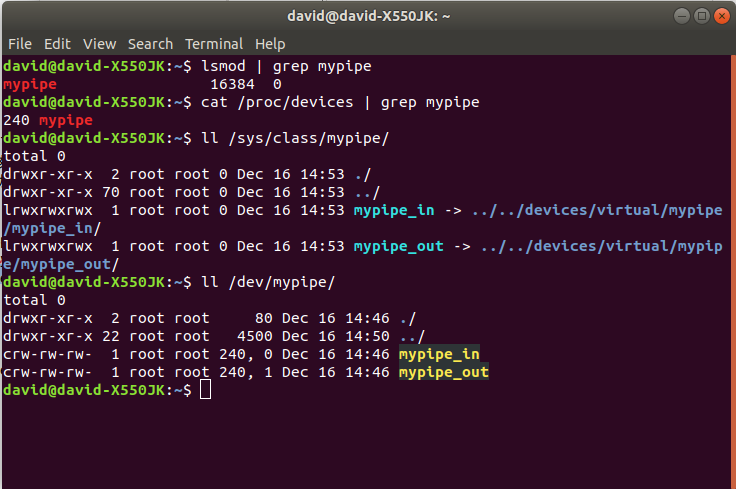
\includegraphics[width=\linewidth]{sh_success.png}
\end{figure}

\subsection{测试}
在bash可以重定向的管道使命令工作。echo写入结束后,cat会在\cinline{read()}时会受到\cinline{-EPIPE}错误,如同在\cinline{dev_read()}中那样。
\begin{figure}[H]
\centering
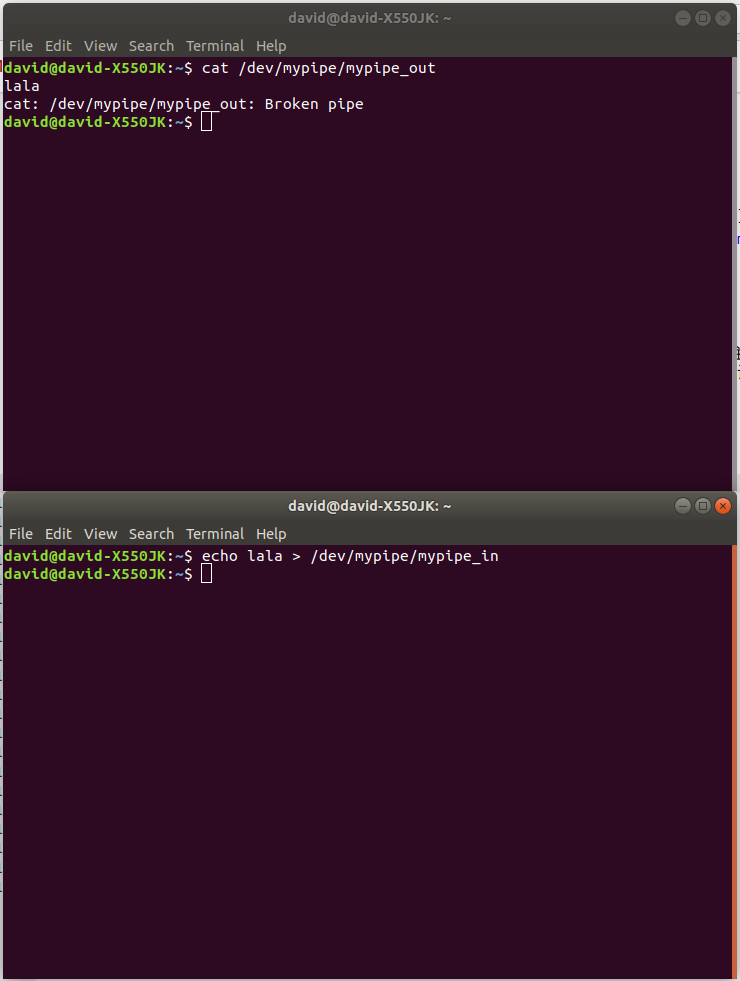
\includegraphics[width=\linewidth]{echo_cat.png}
\end{figure}

编写死循环的读者写者,正常工作。并且其中一个终止后,另一个也会终止。
\begin{figure}[H]
\centering
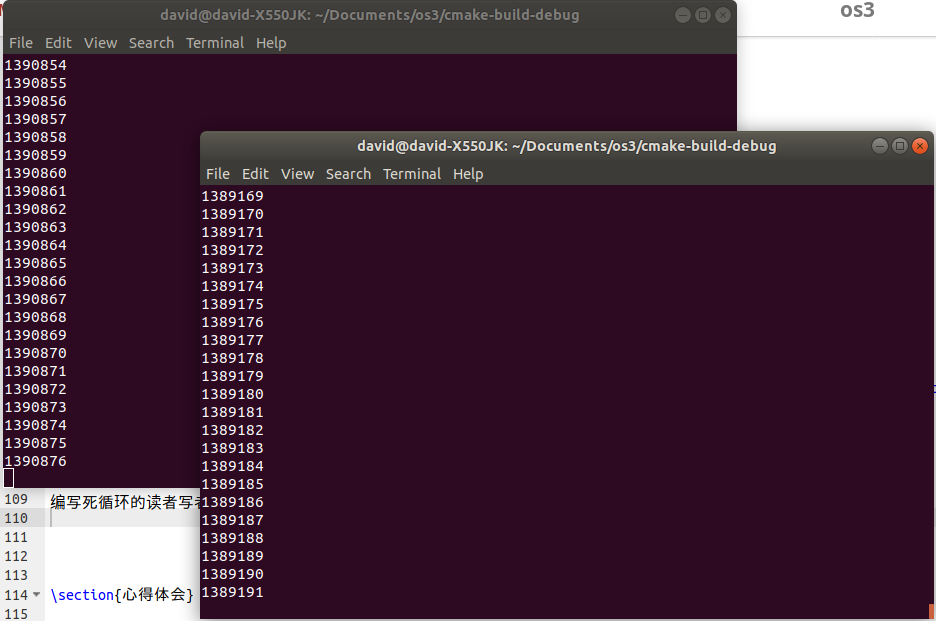
\includegraphics[width=\linewidth]{read_write.png}
\end{figure}

\subsection{系统日志}
编写的内核模块中大量使用了\cinline{printk()},所以系统日志里有大量输出,参加附录\ref{app:log}

\section{心得体会}
\begin{itemize}
    \item 系统级编程跟平时的应用级编程差距较大。我用的CLion平常用起来很方便。但遇到了内核编程风格时完全鬼畜,头文件都认为是错误的。
    \item Linux内核模块编译需要自己写Makefile。动态安装本质上是将模块二进制代码插入内核空间,共享了全局符号表。所以为了避免问题,所有自己的符号都是\cinline{static}的。
    \item 内核编程时用到了大量的宏和嵌套汇编,虽然看不太懂,但还是对OS内部运行机制有了第一手了解,很长见识。
    \item Linux似乎是一个快速迭代但十分向后兼容的系统。就设备驱动这方面,在查资料时就发现了两种差距比较大的形式。一种是\cinline{register_chrdev()}和\cinline{mknod()},直接注册设备号后手动建立设备文件;另一种是我采用的,步骤比较多,但是可以给予更多控制。结构\cinline{class}中成员\cinline{devnode}也是之后才有的,可以在驱动安装时配置好/dev中的设备文件。
    \item 一切在Linux里都视为文件,设备类在/sys/class,设备在/dev,进程信息出现在/proc(似乎/sys跟/proc有重合)。通过自己写代码,对这种Unix哲学有了更深刻的感知。
    \item 系统编程需要区分内核空间和用户空间。大量用户控件显然的东西都不能使用,比如stdio和pthread,需要利用近似的内核的库,有些不顺利。
    \item 不过不管是用户态还是内核态,并行编程大体思路是相通的。内核模块要提供系统调用的实现,而用户应用需求是并发的,所以内核模块需要同步不同部分。
    \item 这里实现了阻塞方式的管道,所以内核模块要处理读写同步的问题,所以使用了两个信号量表征缓存“空”和“满”,最终效果不错。
\end{itemize}

\newpage
\begin{appendix}
\section{驱动模块代码}
\cfile[label=mypipe.c]{mypipe.c}

\section{写者代码}
\cfile[label=writer.c]{writer.c}

\section{读者代码}
\cfile[label=reader.c]{reader.c}

\section{系统日志输出(部分)}
\label{app:log}
\verbatiminput{log}

\end{appendix}
\end{document}

